\documentclass[12pt]{article}
\usepackage{graphicx}
\usepackage{url}
\author{CH22B046}
\title{Virial Equation of State}
\begin{document}
\maketitle
\section{CH22B046}

Name : Abhinandan Jain;
GitHub Username : AbhinandanJain-2004

\subsection{Introduction}
An equation of state is a thermodynamic equation which relates state variables at fixed conditions. These equations are helpful in describing the properties of pure substances or a mixture of substances. After the advent of ideal gas equation, experiments were conducted on different gases. With real gases, a clear deviation was seen. For an ideal gas, compressibility factor is 1, the deviation of real gas from this behaviour is shown in the graph~\ref{Graph}. To remove this inaccuracy, different modifications were made. Virial equation of state is a type of cubic equation of state.

\begin{figure}[ht]
	\begin{center}
		\framebox{
			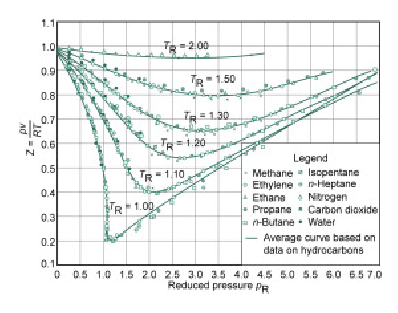
\includegraphics[scale=0.7]{Deviation.eps}
		}
	\end{center}
	\caption{The deviation of real gases from ideal behaviour}
	\label{Graph}
\end{figure}

\subsection{The Equation}
The Virial State of Equation is written as equation~\ref{virial}. Alternatively, it can also be written as equation~\ref{alternative}.

\begin{equation}
	Z = A + \frac{B}{V_m} + \frac{C}{V_m^2} + \frac{D}{V_m^3} + . . .
	\label{virial}
\end{equation}

\begin{equation}
	Z = A + B\rho + C{\rho}^2 + D{\rho}^3 + . . .
	\label{alternative}
\end{equation}

where, $Z$ is the compressibility factor, given by equation~\ref{Z}.

\begin{equation}
	Z = \frac {pV_m} {RT}
	\label{Z}
\end{equation}
This equation is one of the most general function directly derived from statistical mechanics.

The coefficients A, B, C,... are called the virial coefficients. The value of virial coefficients can be found as a function of intermolecular forces. The first Virial coefficient, $A$ has a constant value of 1. This tells that at low densities or high volumes, all fluids act as an ideal gas. The second virial coefficient $B$ corresponds to interactions between two molecules, $C$ between triplets, and so on~\cite{enwiki:1153405425}. These virial coefficients $B,C,D,...$ are functions of temperature only and are generally presented as a Taylor Series in terms of $\frac{1}{T}$ as taken from~\cite{enwiki:1141609317}

\bibliography{Ref.bib}
\bibliographystyle{plain}
\end{document}